\documentclass[11pt]{beamer}
\usepackage[T1]{fontenc}
\usepackage[utf8]{vietnam}
\usepackage{hyperref}
\usepackage{url}
\usepackage{xcolor}
\usepackage[linesnumbered, ruled, longend]{algorithm2e}
\usepackage{colortbl}
\usepackage{subcaption}
\usepackage{amsmath,amssymb}
\usepackage{ragged2e}
\usepackage{multirow}
\usepackage{changepage}
\setbeamerfont{frametitle}{size=\large}
\usepackage{caption}
\captionsetup{labelformat=empty}
\usepackage{booktabs}
\usepackage{array}
\newcolumntype{P}{>{\centering\arraybackslash}p}
%\usepackage{enumitem}
% \usepackage[table,xcdraw]{xcolor}
% \usepackage{etoolbox}
\renewcommand{\raggedright}{\leftskip=0pt \rightskip=0pt plus 0cm}
\apptocmd{\frame}{}{\justifying}{}
\let\oldenumerate=\enumerate 
\renewenvironment{enumerate}{\oldenumerate\raggedright}{\endlist} 
\let\olditemize=\itemize
\renewenvironment{itemize}{\olditemize\raggedright}{\endlist}

\usepackage{xcolor}
\definecolor{commentgreen}{RGB}{2,112,10}
\definecolor{eminence}{RGB}{108,48,130}
\definecolor{weborange}{RGB}{255,165,0}
\definecolor{frenchplum}{RGB}{129,20,83}

\usepackage{listings}
\usepackage{textcomp}
\lstset {
	language=Java,
	frame=tb,
	tabsize=4,
	showstringspaces=false,
	numbers=left,
	upquote=true,
	commentstyle=\color{commentgreen},
	keywordstyle=\color{eminence},
	stringstyle=\color{red},
	basicstyle=\small\ttfamily, % basic font setting
	emph={int,char,double,float,unsigned,void,bool},
	emphstyle={\color{blue}},
	escapechar=\&,
	% keyword highlighting
	classoffset=1, % starting new class
	morekeywords={>,<,.,;,,,-,!,=,~},
	keywordstyle=\color{weborange},
	classoffset=0,
}

\usepackage{adjustbox}
\newcommand{\code}[1]{\texttt{#1}}

\usetheme{Warsaw}
\useoutertheme{smoothtree}
\usepackage[utf8]{vietnam}
%%%%%%%%%%%%%%%%%%%%%%%%%%%%%%%%%%%%
\def\mydate{\leavevmode\hbox{\bfseries\the\day/\twodigits\month/\twodigits\year}}
\def\twodigits#1{\ifnum#1<10 0\fi\the#1}
%%%%%%%%%%%%%%%%%%%%%%%%%%%%%%%%%%%%
\definecolor{sectioncolor}{RGB}{39,0,118}
\definecolor{framecolor}{RGB}{37,109,255}

\setbeamercolor{frametitle}{fg=white, bg=blue}
\definecolor{light-gray}{gray}{0.95}
%%%%%%%%%%%%%%%%%%%%%%%%%%%%%%%%%%%
\setbeamertemplate{footline}
{%
	\leavevmode%
	\begin{beamercolorbox}[wd=.5\paperwidth,ht=2.75ex,dp=1.5ex]{author in head/foot}%
		\hbox to .5\paperwidth{\hfil\insertshortauthor\hfil}
	\end{beamercolorbox}%
	\begin{beamercolorbox}[wd=.5\paperwidth,ht=2.75ex,dp=1.5ex]{date in head/foot}%
		\raggedleft
		\usebeamerfont{date in head/foot}
		\insertframenumber{} / \inserttotalframenumber\hspace*{15pt}
	\end{beamercolorbox}%
}
%==============================================
\makeatletter
\patchcmd{\beamer@sectionintoc}
{\vfill}
{\vskip\itemsep}
{}
{}
\makeatother  
\begin{document}
\captionsenglish
\dateUSenglish
\author[Le Vu Loi]{
	\begin{center}
		{\fontsize{14pt}{\baselineskip}\selectfont Le Vu Loi - 20173240} \\[10pt]
		{\fontsize{12pt}{\baselineskip}\selectfont Talented class of Computer Science} \\[25pt]
		\textbf{Supervisor}: Assoc. Prof. Pham Van Hai\\
		Department of Information System
	\end{center}
	%	\begin{tabular}{ll}
	%		Le Vu Loi - 20173240 \\[]
	%		
	%		\textit{Supervisor} & Assoc. Prof. Pham Van Hai
	%	\end{tabular}
}
\title[]{\bfseries\fontsize{14}{\baselineskip}\selectfont BACHELOR THESIS\vspace{5pt}}
\subtitle{The proposed Dual Encoder model for Open-domain
	question answering system: Case study in Vietnamese
	COVID-19 topic}
\logo{
\includegraphics[scale=.1]{images/SoICTlogo.jpg}}
\institute[\bfseries Viện CNTT\&TT]{}
\date[\mydate]{\today}
%\subject{Yo!}
\begin{frame}[plain]
	\maketitle
\end{frame}
%====================================================
\begin{frame}[plain]
\begin{itemize}
	\item Kính thưa thầy Chủ tịch Hội đồng và các thầy cô trong hội đồng, thưa toàn thể các bạn. Em là Lê Vũ Lợi, sinh viên lớp Tài năng Công nghệ thông tin K62. Hôm nay em xin trình bày đồ án tốt nghiệp của mình với tên đề tài là "The proposed Dual Encoder model for Open-domain question answering system: Case study in Vietnamese COVID-19 topic". Đề tài được thực hiện dưới sự hướng dẫn của PGS.TS. Phạm Văn Hải. Sau đây em xin được bắt đầu.
\end{itemize}
\end{frame}
%====================================
\begin{frame}[plain]
	\frametitle{Outline}
	\begin{columns}[t]
		\begin{column}{.5\textwidth}
			\tableofcontents[sections={1-3}]
		\end{column}
		\begin{column}{.5\textwidth}
			\tableofcontents[sections={4-6}]
		\end{column}
	\end{columns}
\end{frame}
\begin{frame}
	\begin{itemize}
		\item Bố cục phần trình bày của em gồm có 5 phần: thứ nhất là phần giới thiệu tổng quan, thứ 2 là các nghiên cứu liên quan, thứ 3 là mô hình đề xuất, thứ 4 là áp dụng mô hình nghiên cứu cho dữ liệu tiếng Việt. Thứ 5 là kết quả thực nghiệm và cuối cùng là kết luận và hướng phát triển.
	\end{itemize}
\end{frame}
%====================================
\section{Introduction}
\subsection{Overview}
\begin{frame}
	\frametitle{Open-domain question answering}
	\hspace*{-15pt}
	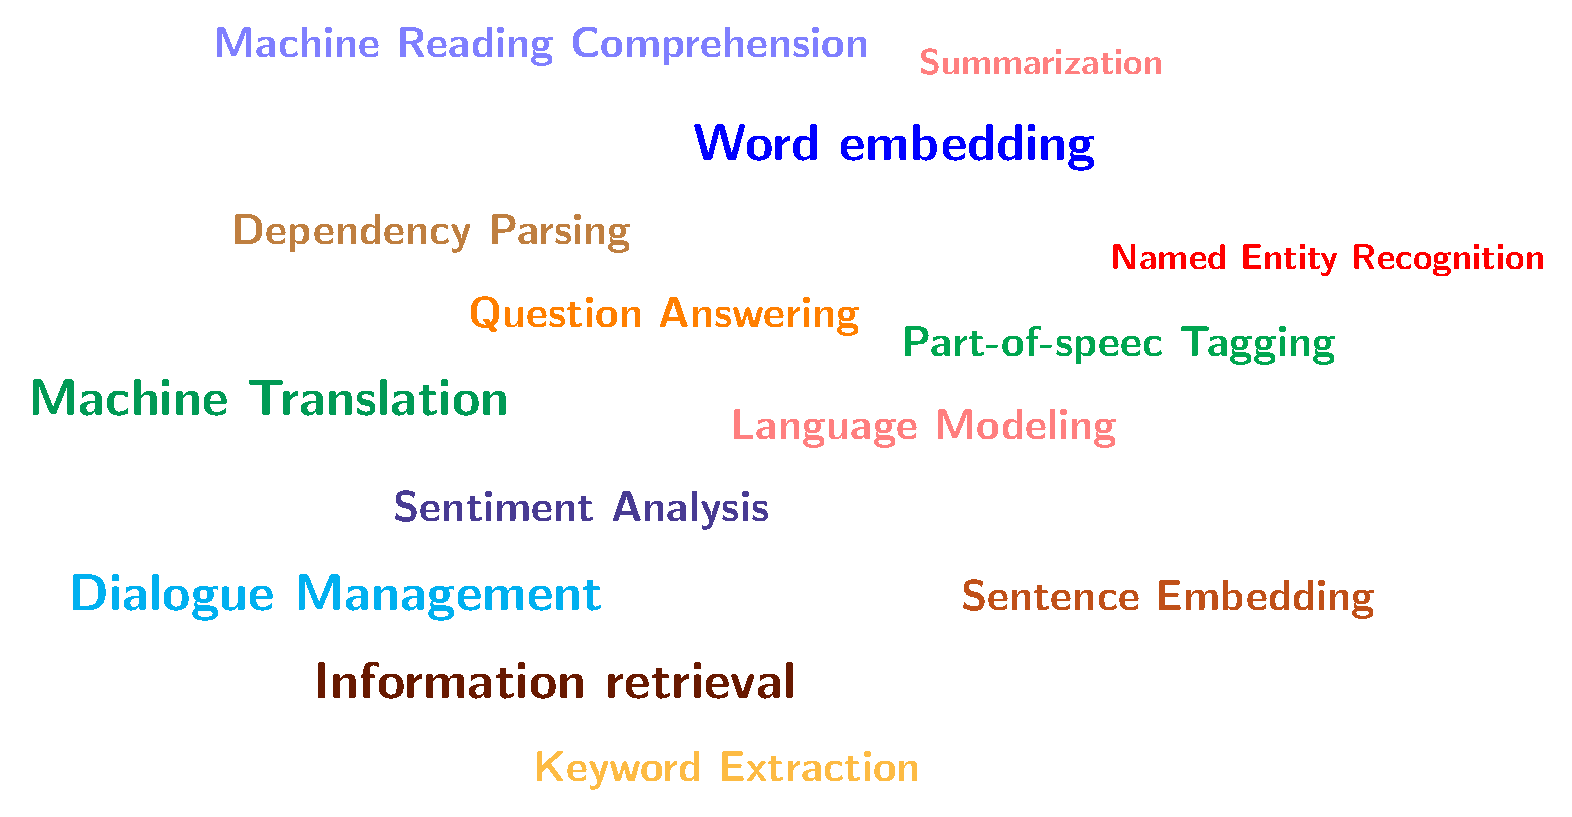
\includegraphics[scale=.45]{images/PDF/nlptask/nlptask.pdf}
\end{frame}
\begin{frame}
	\begin{itemize}
		\item Em xin đi vào phần đầu tiên là giới thiệu tổng quan.
		\item Bài toán em nghiên cứu mang tên là Open-domain question answering (hệ thống trả lời câu hỏi miền mở)
		\item Đây là một bài toán ở mức độ tương đối khó trong lĩnh vực xử lý ngôn ngữ tự nhiên, nó dựa trên các bài toán nền tảng hơn như: word embedding,language modeling, question answering, information retrieval hay machine reading comprehension.
	\end{itemize}
\end{frame}
%====================================
%\begin{frame}
%\frametitle{Open-domain question answering}
%\textbf{Open-domain question answering is at medium level of difficulty among various NLP tasks.} \\[10pt]
%\begin{itemize}
%\item Word embedding
%\item Sentence embedding
%\item Language Modeling \\
%.....
%\item Question Answering
%\item \textcolor{blue}{\bfseries Open-domain question answering}\\
%.....
%\item Text Summarization
%\item Dialogue Management
%\end{itemize}
%\end{frame}
%====================================
\begin{frame}
	\frametitle{Open-domain question answering}
	%\vspace{-.5cm}
	\begin{itemize}
		\item Combination of \textbf{retriever} (Information Retrieval) and \textbf{reader} (Machine Reading Comprehension)
		\begin{itemize}
			\item "Skim through" a large data source to find a subset of relevant documents.
			\item "Swallow" each document to find the exact answer(s).
		\end{itemize}
	\end{itemize}
	%\hspace*{-15pt}
	%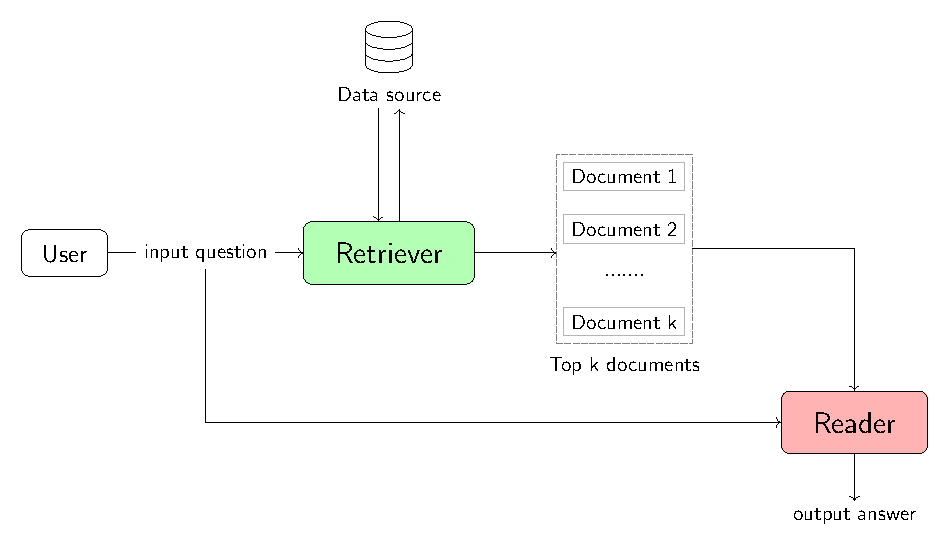
\includegraphics[scale=.68]{images/PDF/overall_arch/architecture.pdf}
\end{frame}
\begin{frame}
\begin{itemize}
	\item Cụ thể hơn thì có thể xem bài toán open-domain question answering là sự kết hợp của bài toán information retrieval và machine reading comprehension.
	\item Trong đó, thành phần retriever sẽ thực hiện tìm kiếm sơ bộ trên một kho văn bản kích thước lớn có sẵn để lọc ra một tập nhỏ các văn bản liên quan nhất tới một câu hỏi của người dùng
	\item Tiếp đó, thành phần reader có nhiệm vụ đọc kĩ tập văn bản này để tìm ra câu trả lời chính xác nhất
\end{itemize}
\end{frame}
%====================================
\subsection{Problem formulation}
\begin{frame}
	\begin{adjustwidth}{-2em}{1em}
		\frametitle{Problem formulation}
		\begin{itemize}
			\item \textbf{Input} 
			\begin{itemize}
				\item A question in human natural language.\\[5pt]
				\textit{E.g.} Who is the founder of Google?
			\end{itemize}
			\item \textbf{Output}
			\begin{itemize}
				\item A list of answers for the input question \\[5pt]
				\textit{E.g.} [Larry Page, Sergey Brin]
			\end{itemize}
			\item \textbf{Constraints}
			\begin{itemize}
				\item The system answers only factoid question.
				%		\item Factoid question means that the question is about a fact and often can be answered by a short phrase. Yes/no question, multiple-choice question and reasoning question are not factoid. \\[5pt]
				%		- \textit{Factoid question}: What is the capital of Vietnam? \\
				%		- \textit{Reasoning question}: If 3 cats can catch 3 mice in 3 minutes, how many mices can 6 cats catch in 6 minutes?
			\end{itemize}
			%\begin{figure}
			%	content...
			%\end{figure}
		\end{itemize}
	\end{adjustwidth}
\end{frame}
\begin{frame}
\begin{itemize}
	\item Phát biểu bài toán Open-domain question answering
	\item Bài toán nhận đầu vào là một câu hỏi của người dùng dưới dạng ngôn ngữ tự nhiên, đầu ra của bài toán là một hoặc một danh sách các câu trả lời tương ứng với câu hỏi đã cho. Ràng buộc của bài toán là hệ thống chỉ trả lời các câu hỏi có tính chất factoid
	\item Một câu hỏi có tính chất factoid nếu nó liên quan đến một sự thật hiển nhiên. Ví dụ như câu hỏi "Thành phố nào là thủ đô của Việt Nam". Ví dụ về câu hỏi không có tính chất factoid đó là câu "Tại sao anh ta không thích làm điều này". Câu hỏi này phụ thuộc vào một ngữ cảnh cụ thể nên không có tính chất factoid. Các câu hỏi dạng yes/no, câu hỏi trắc nghiệm hay câu hỏi suy diễn cũng không thuộc dạng câu hỏi factoid.
\end{itemize}
\end{frame}
%====================================
\section{Related works}
\begin{frame}
	\frametitle{Related works}
	\begin{thebibliography}{10}
		\bibitem{mrc}
		[1] Danqi Chen, Adam Fisch, Jason Weston, and Antoine Bordes. Reading wikipedia to answer open-domain questions. \underline{arXiv preprint arXiv:1704.00051}, 2017.
		\bibitem{dpr}
		[2] Vladimir Karpukhin, Barlas Oguz, Sewon Min, Patrick Lewis, Ledell Wu, Sergey Edunov, Danqi Chen, and Wen-tau Yih. Dense passage retrieval for open-domain	question answering. \underline{arXiv preprint arXiv:2004.04906}, 2020.
	\end{thebibliography}
\end{frame}
\begin{frame}
	\begin{itemize}
		\item Phần thứ hai em xin trình bày về các nghiên cứu liên quan
	\end{itemize}
\end{frame}
%====================================
\begin{frame}
	\frametitle{Reading Wikipedia to answer open-domain questions}
	\begin{itemize}
		%	\item Danqi Chen et. al \cite{mrc} proposed to solve open-domain question answering problem by reading Wikipedia to find answers.
		%	\item Consist of a \textbf{document retriever} based on bigram hashing and TF-IDF matching and \textbf{machine reader} based on multi-layer Recurrent neural network.Chen et. al \cite{mrc} proposed to solve open-domain question answering problem by reading Wikipedia to find answers.
		%\item Consist of a \textbf{document retriever} based on bigram hashing and TF-IDF matching and \textbf{machine reader} based on multi-layer Recurrent neural network.
		%\item This work promoted a large number of subsequent publications on Open-domain question answering problem.
		%	\item This work promoted a large number of subsequent publications on Open-domain question answering problem.
		\item \textbf{Retriever}: bigram hashing and TF-IDF matching
		\item \textbf{Reader}: Multi-layer recurrent neural network
		\item Potential improvements: using neural network to better capture documents' semantics
	\end{itemize}
\end{frame}
\begin{frame}
\begin{itemize}
	\item Nghiên cứu thứ nhất mang tên "Reading wikipedia to answer open-domain question answering"
	\item Nghiên cứu sử dụng thuật toán bigram hashing và TF-IDF matching cho thành phần retriever và mạng hồi quy nhiều tầng cho thành phần reader.
	\item Nghiên cứu này đã đánh dấu một cột mốc trong các nghiên cứu về bài toán ODQA và thu hút sự chú ý của một loạt các nghiên cứu sau đó đối với cùng chủ đề.
	\item Một hướng cải thiện tiềm năng cho nghiên cứu này đó là sử dụng deep learning cho thành phần retriever để mô hình có thể bắt được ngữ nghĩa của các văn bản một cách tốt hơn.
\end{itemize}
\end{frame}
%====================================
\begin{frame}
	\frametitle{Dense passage retrieval}
	\begin{itemize}
		%	\item Karpukhin et. al \cite{dpr} proposed to use a dense retriever which based on Dual encoder architecture for retrieving documents in open-domain question answering system.
		%	\item Dual encoder consists of a question encoder and a context encoder, which is used to encode question and document respectively into (a) vector space(s).
		%	\item Similarity between a document and a question is computed by taking dot product of the encoded question and the encoded document.
		%	\item Relevant documents to the input question are retrieved using this similarity.
		\item \textbf{Retriever}: Dual-encoder
		\item \textbf{Reader}: Cross-encoder
		\item Successfully use neural network to solve information retrieval.
		\item Potential improvements: More challenging learning task for the system to gain deeper language understanding.
	\end{itemize}
\end{frame}
\begin{frame}
\begin{itemize}
	\item Nghiên cứu sử dụng kiến trúc dual encoder cho thành phần retriever và kiến trúc cross-encoder cho thành phần reader. Đây là các kiến trúc mạng nơ ron được sử dụng gần đây trong lĩnh vực xử lý ngôn ngữ tự nhiên.
	\item Nghiên cứu này lần đầu tiên sử dụng deep learning cho bài toán Informational retrieval và kết quả thu được vượt xa so với hướng tiếp cận truyền thống không sử dụng deep learning.
	\item Một hướng cải thiện tiềm năng cho nghiên cứu này đó là sử dụng mục tiêu học khó hơn để thách thức mô hình và giúp mô hình đạt được mức độ hiểu ngôn ngữ sâu hơn.
\end{itemize}
\end{frame}
%====================================
\section{Proposed method}
\subsection{System pipeline}
\begin{frame}
	\frametitle{System pipeline}
	\begin{itemize}
		\item Open-domain question answering = Retriever + Reader
	\end{itemize}
	\hspace*{-15pt}
	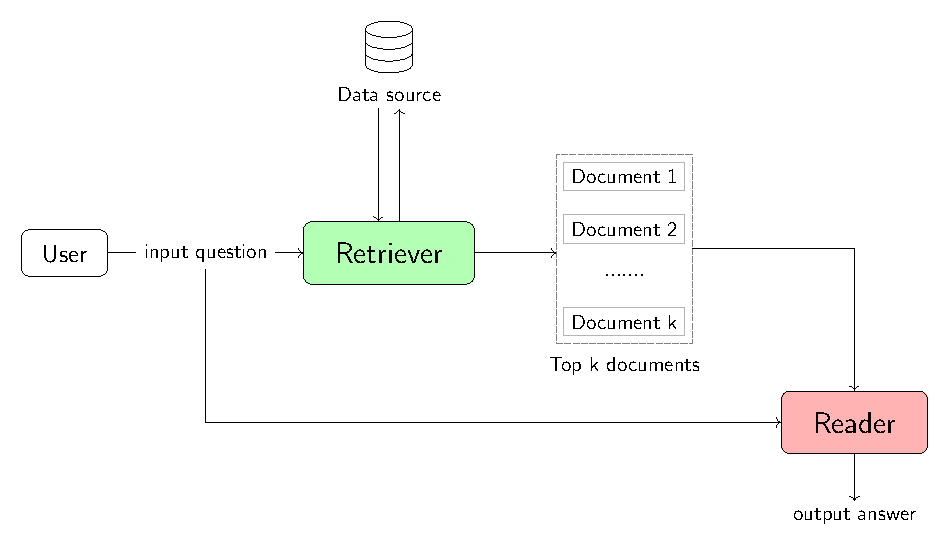
\includegraphics[scale=.68]{images/PDF/overall_arch/architecture.pdf}
\end{frame}
\begin{frame}
\begin{itemize}
	\item Phần thứ 3 của bài trình bày em xin đi vào mô hình đề xuất
	\item Trước tiên, em sẽ trình bày về kiến trúc tổng quan của hệ thống open-domain question answering.
	\item Hệ thống gồm 2 thành phần chính là retriever và reader.
	\item Thành phần retriever có nhiệm vụ tìm kiếm trong một kho văn bản với kích thước lớn để tìm ra một tập con các văn bản có liên quan nhất tới câu hỏi đầu vào của người dùng
	\item Thành phần reader có nhiệm vụ đọc các văn bản trả về bởi retriever và tìm ra câu trả lời chính xác
\end{itemize}
\end{frame}
%====================================
\subsection{Retriever}
\begin{frame}
	\frametitle{Dense retriever: Dual encoder architecture}
	\begin{itemize}
		\item Dense retriever is based on Dual encoder architecture.
	\end{itemize}
	\begin{figure}[h]
		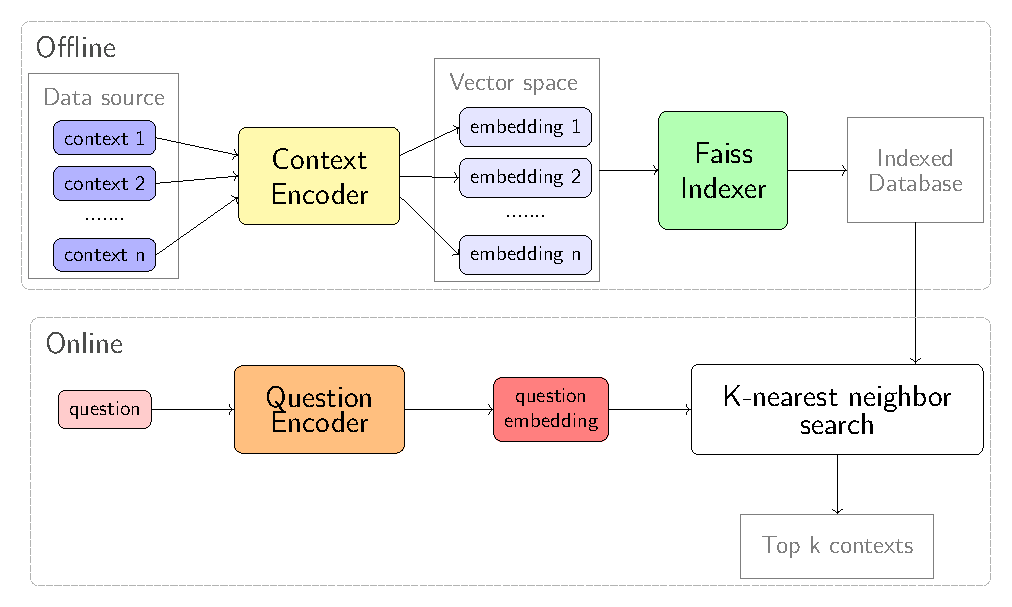
\includegraphics[scale=.57]{images/PDF/biencoder/biencoder.pdf}
		\caption{Workflow of a dense retriever}
	\end{figure}
\end{frame}
\begin{frame}
\begin{itemize}
	\item Em sẽ đi vào thành phần đầu tiên là retriever. Thành phần này dựa trên kiến trúc dual encoder, bao gồm 2 mạng mã hóa độc lập là Context Encoder và Question Encoder.
	\item Như thể hiện trên hình vẽ thì luồng làm việc của retriever bao gồm 2 pha. Ở pha offline, mạng context encoder sẽ mã hóa tất cả các văn bản trong kho văn bản thành các vector trong không gian vector. Các vector này sau đó được đánh chỉ mục để phục vụ việc tìm kiếm nhanh ở pha online.
	\item Ở pha online, khi người dùng đưa ra một câu hỏi thì hệ thống sẽ sử dụng thành phần question encoder để mã hóa câu hỏi thành vector question embedding. Vector này sau được tìm kiếm trên kho văn bản mã hóa đã được đánh chỉ mục để trả về top-k văn bản có liên quan nhất đến câu hỏi người dùng.
\end{itemize}
\end{frame}
%====================================
\begin{frame}
	\frametitle{Training dense retriever}
	\begin{itemize}
		\item Jointly train question encoder and context encoder.
		\item Training data: a training sample consists of:
		\begin{itemize}
			\item $q$: input question.
			\item $p^+$: positive context, which is the document that contains the answers.\\[5pt]
			\item $\left\{p^-_j\right\}_{j=1}^m$: $m$ negative contexts, which are documents that do not contain the answers.
		\end{itemize}
		\item Loss function (per one training sample): negative log-likelihood
		\begin{equation}
			\label{eq:01}
			\mathcal{L} = -\log\left\{\dfrac{\exp\left[{\text{sim}\left(q, p^+\right)}\right]}{\exp\left[{\text{sim}\left(q, p^+\right)}\right] + \sum\limits_{j=1}^m \exp\left[{\text{sim}\left(q, p^-_j\right)}\right]}\right\}
		\end{equation}
	\end{itemize}
\end{frame}
\begin{frame}
	\begin{itemize}
		\item Để huấn luyện thành phần retriever, ta thực hiện tối ưu đồng thời 2 mạng question encoder và context encoder.
		\item Một mẫu dữ liệu sử dụng huấn luyện retriever bao gồm một câu hỏi, một văn bản positive (tức là văn bản chứa câu trả lời tương ứng với câu hỏi đã cho) và $m$ văn bản negative, là các văn bản không chứa câu trả lời cho câu hỏi đã cho.
		\item Hàm loss sử dụng là hàm negative log likelihood. Hàm này cố gắng cực đại hóa độ tương đồng giữa câu hỏi đầu vào với văn bản positive, đồng thời cực tiểu hóa độ tương đồng giữa câu hỏi với các văn bản negative.
		%	\item 
	\end{itemize}
\end{frame}
%====================================
\subsection{Reader}
\begin{frame}
	\frametitle{Extractive reader: Cross encoder architecture}
	\begin{itemize}
		\item Extractive reader's task is to predict the start and end position of answer in the documents returned by dense retriever.\\
		\begin{center}
			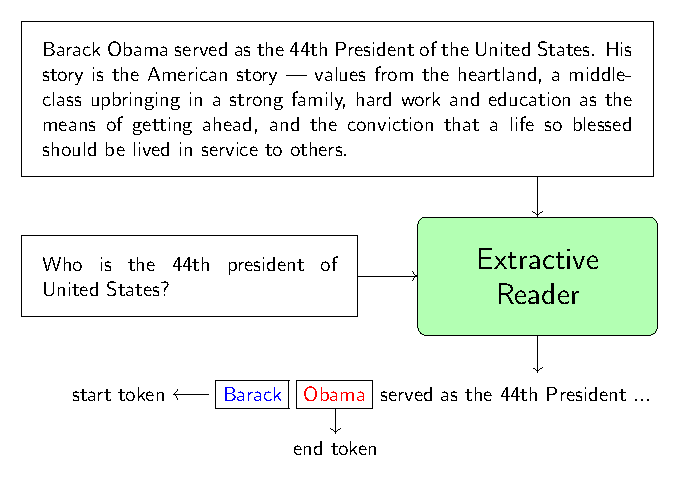
\includegraphics[scale=.55]{images/PDF/extractive_reader/extractive_reader.pdf}
		\end{center}
		\item Extractive reader consists of 2 components, in which each component follows a cross encoder architecture:
		\begin{itemize}
			\item Re-ranker: re-rank documents returned by dense retriever.
			\item Single-document reader: read one document to extract answers.
		\end{itemize}
	\end{itemize}
\end{frame}
\begin{frame}
\begin{itemize}
\item {\fontsize{9pt}{\baselineskip}\selectfont Thành phần thứ 2 của hệ thống là reader. Cụ thể đồ án của em sử dụng extractive reader. Extractive ở đây có nghĩa là reader sẽ trích xuất ra câu trả lời từ văn bản nó đang đọc, đồng nghĩa với việc câu trả lời phải là một cụm từ nằm trong văn bản, một ví dụ được đưa ra như hình ảnh trên slide. Một loại reader khác cũng được cộng đồng nghiên cứu quan tâm mang tên là generative reader. Đối với loại này thì câu trả lời không bị ràng buộc phải nằm trong văn bản mà mô hình có thể sinh ra bất kỳ câu trả lời nào mà nó nghĩ là hợp lý nhất. Tuy nhiên loại reader này đòi hỏi số lượng tham số lớn cũng như đặt ra nhiều thách thức hơn trong việc huấn luyện.}
\item {\fontsize{9pt}{\baselineskip}\selectfont Đối với thành phần reader thì em lại chia nhỏ thành 2 thành phần con đó là re-ranker và single-document reader. Thành phần re-ranker có nhiệm vụ sắp xếp lại thứ hạng của các văn bản trả về bởi retriever và sau đó thành phần single-document reader sẽ đọc các văn bản được xếp hạng bởi re-ranker theo thứ tự từ trên xuống dưới.}
\end{itemize}
\end{frame}
%====================================
\begin{frame}
	\frametitle{Re-ranker}
	\vspace*{-20pt}
	\begin{figure}[h]
		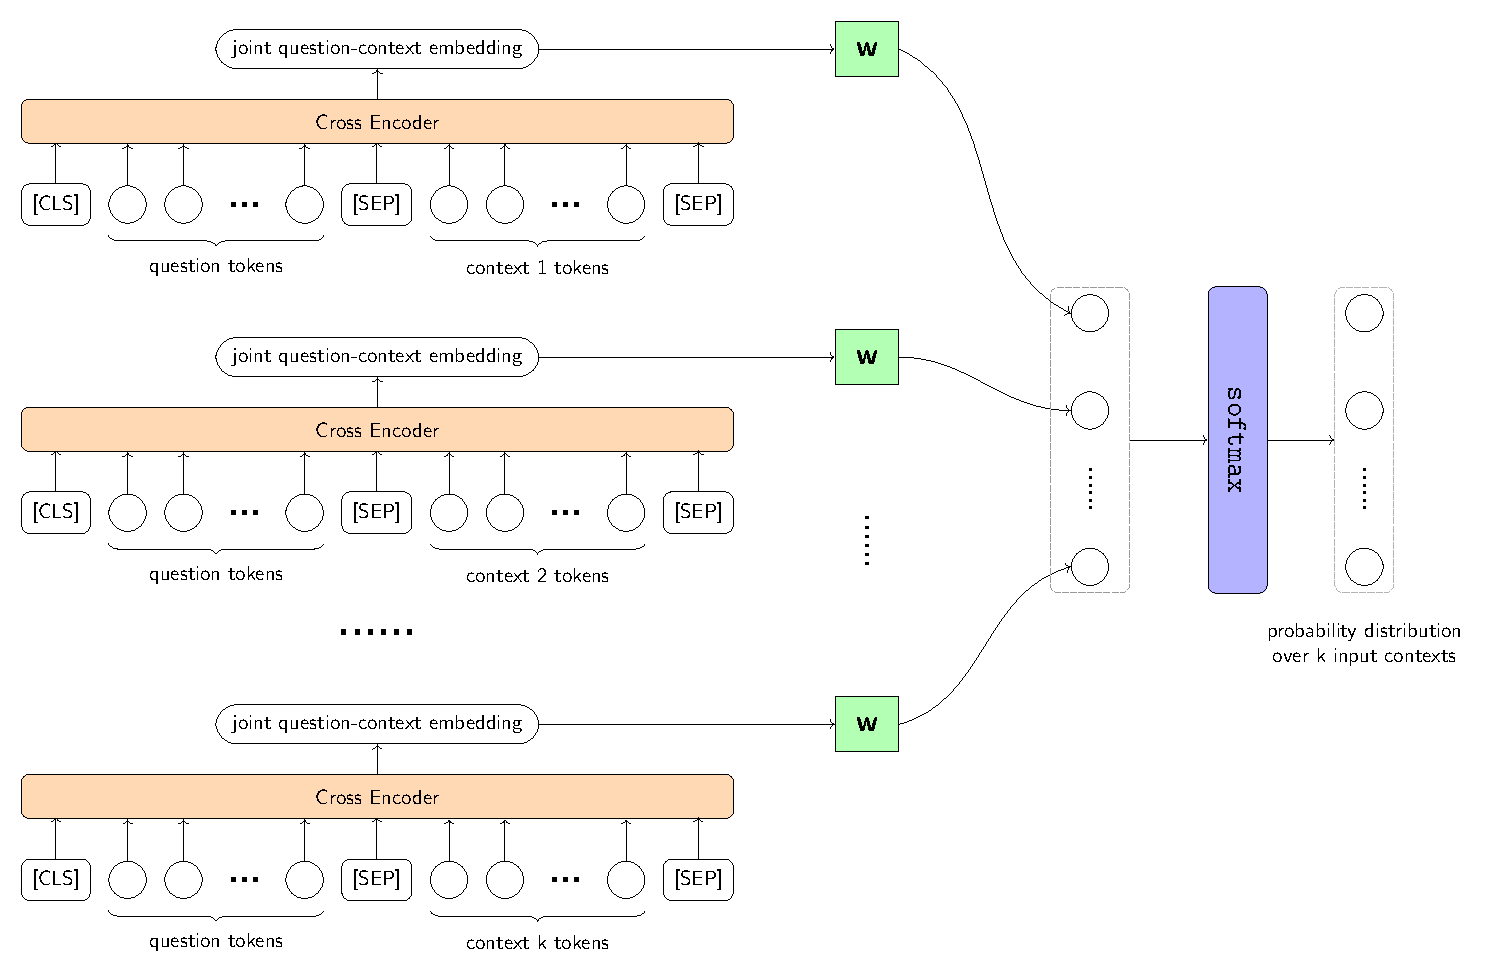
\includegraphics[scale=.43]{images/PDF/full-reranker/fullRerank.pdf}
		\caption{Model architecture}
	\end{figure}
\end{frame}
\begin{frame}
\begin{itemize}
	\item {\fontsize{8pt}{\baselineskip}\selectfont Slide này trình bày kiến trúc của thành phần re-ranker. Re-ranker tuân theo kiến trúc cross-encoder, nhận đầu vào là k chuỗi ghép nối giữa câu hỏi đầu vào và k văn bản đang cần được xếp hạng. Mỗi chuỗi này sau khi đi qua mạng cross-encoder sẽ trả về một vector mã hóa đồng thời cho câu hỏi và văn bản. Vector này sau đó được nhân với một ma trận w và trả về một score tương ứng với khả năng mà văn bản tương ứng là văn bản chứa câu trả lời. Cuối cùng k score này được chuẩn hóa bằng hàm softmax để trả về một phân phối xác suất ứng với xác suất một văn bản có chứa câu trả lời.}
\end{itemize}
\end{frame}
%====================================
%\begin{frame}
%\frametitle{Training re-ranker}
%\begin{adjustwidth}{-2em}{0em}
%\begin{itemize}
%	\item {\fontsize{10pt}{\baselineskip}\selectfont Target to maximize probability of positive context over negative contexts.}
%	\item {\fontsize{10pt}{\baselineskip}\selectfont Training data: a training sample consists of:}
%	\begin{itemize}
%		\item {\fontsize{9pt}{\baselineskip}\selectfont$q$: input question.}
%		\item {\fontsize{9pt}{\baselineskip}\selectfont$p^+$: positive context.}
%		\item {\fontsize{9pt}{\baselineskip}\selectfont$\left\{p_j^-\right\}_{j=1}^m$: $m$ negative contexts.}
%	\end{itemize}
%	\item {\fontsize{10pt}{\baselineskip}\selectfont Loss function}
%	\begin{itemize}
%		\item {\fontsize{9pt}{\baselineskip}\selectfont Assumptions}
%		\begin{itemize}
%			\item {\fontsize{8pt}{\baselineskip}\selectfont$e^+$: joint question-context embedding vector of input question and positive context.}
%			\item {\fontsize{8pt}{\baselineskip}\selectfont$\left\{e_j^-\right\}_{j=1}^m$: $m$ joint question-context embedding vectors of input question and negative contexts.}
%		\end{itemize}
%	\item {\fontsize{9pt}{\baselineskip}\selectfont Loss formula}
%	\begin{scriptsize}
%	\begin{equation}
%		\label{eq:02}
%		\mathcal{L} = -\log\left\{\dfrac{\exp\left(e^+\mathbf{w}\right)}{\exp\left(e^+\mathbf{w}\right) + \sum\limits_{j=1}^m\exp\left(e_j^-\mathbf{w}\right)}\right\}
%	\end{equation}
%	where $w$ is a learnable vector.
%	\end{scriptsize}
%	\end{itemize}
%\end{itemize}
%\end{adjustwidth}
%\end{frame}
%====================================
\begin{frame}
	\frametitle{Single-document reader}
	\vspace*{-10pt}
	\begin{figure}[h]
		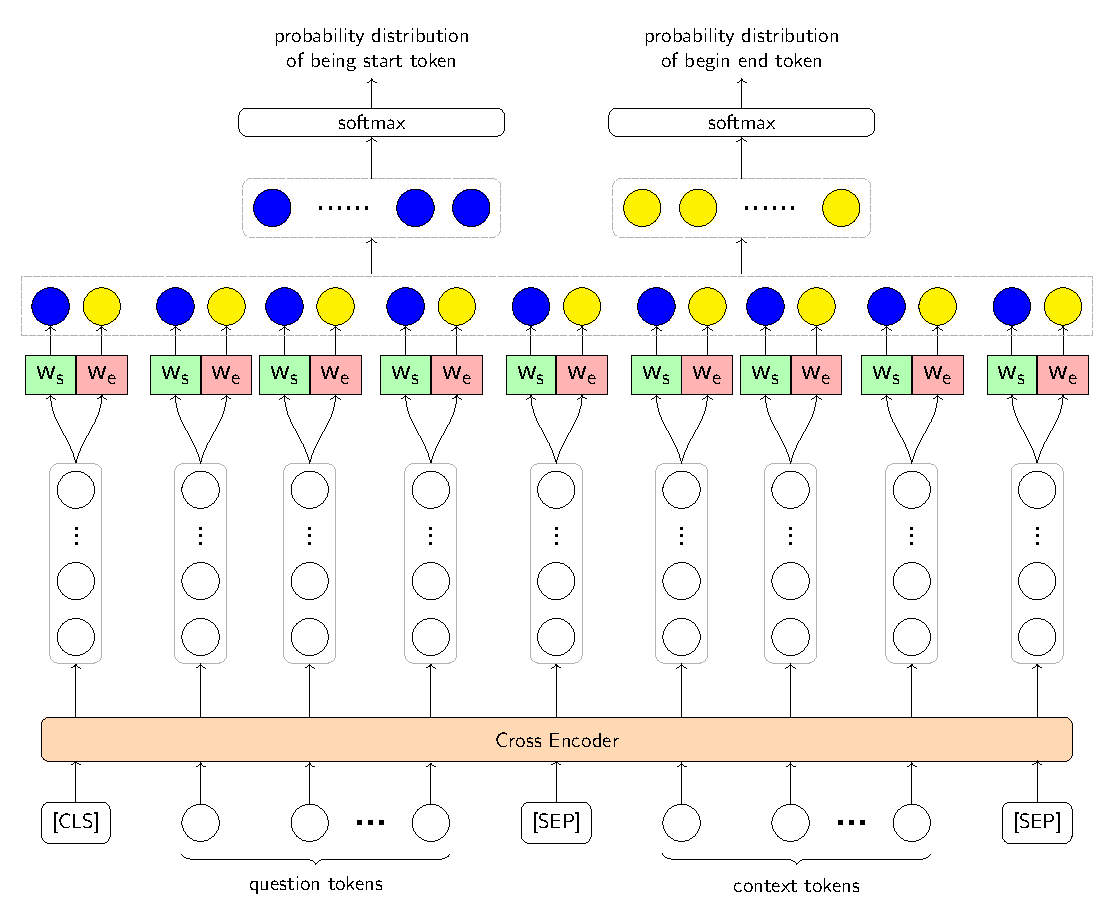
\includegraphics[scale=.45]{images/PDF/singleDocReader/singleDocReader.pdf}
		\caption{Model architecture}
	\end{figure}
\end{frame}
\begin{frame}
\begin{itemize}
	\item {\fontsize{8pt}{\baselineskip}\selectfont Tiếp đến là kiến trúc của thành phần single-document reader. Tương tự như thành phần re-ranker, single-document reader cũng tuân theo kiến trúc cross encoder. Thay vì xử lý đồng thời k chuỗi đầu vào thì single-document chỉ xử lý một chuỗi đầu vào, là ghép nối giữa câu hỏi của người dùng với văn bản mà single-document reader đang xử lý. Mỗi một token trong chuỗi đầu vào được mã hóa thành một vector và vector này sau đó được nhân lần lượt với các ma trận ws, we để sinh ra 2 score tương ứng với khả năng token đang xét là vị trí bắt đầu hay vị trí kết thúc của câu trả lời (2 score được biểu diễn bằng các hình tròn màu xanh dương và màu vàng như trên hình vẽ). Tương tự re-ranker, 2 score này cũng được chuẩn hóa qua hàm softmax để sinh ra 2 phân phối xác suất tương ứng với xác suất token đang xét là vị trí bắt đầu hay kết thúc của câu trả lời.}
\end{itemize}
\end{frame}
%====================================
%\begin{frame}
%\frametitle{Training single-document reader}
%%\begin{adjustwidth}{-2em}{0em}
%\begin{itemize}
%	\item {\fontsize{10pt}{\baselineskip}\selectfont Target to maximize joint probability of answer's start and end position.}
%	\item {\fontsize{10pt}{\baselineskip}\selectfont Training data: a training sample consists of:}
%	\begin{itemize}
%		\item $L$: concatenation of input question and a positive context.
%		\item $s$: start position of the answer.
%		\item $e$: end position of the answer.
%	\end{itemize}
%	\item {\fontsize{10pt}{\baselineskip}\selectfont Loss function}
%	\begin{itemize}
%		\item Assumptions
%		\begin{itemize}
%%			\item $h$: joint question-context embedding vector.
%			\item $\alpha$: probability distribution of being start position.
%			\item $\beta$: probability distribution of being end position.
%		\end{itemize}
%		\item Loss function
%		\begin{equation}
%			\label{eq:03}
%			\mathcal{L} = -\log{\alpha[s]} -\log{\beta[e]}
%		\end{equation}
%	\end{itemize}
%\end{itemize}
%%\end{adjustwidth}
%\end{frame}
%====================================
\subsection{Stratified loss}
%\begin{frame}
%\frametitle{Existing approach: in-batch loss}
%\begin{adjustwidth}{-2em}{0em}
%\begin{itemize}
%	\item Karpukhin et. al \cite{dpr} proposed to use in-batch strategy and hard negative contexts to train dense retriever using negative log-likelihood loss defined in equation~\eqref{eq:01}. To be specific:
%	\begin{itemize}
%		\item In-batch strategy: training samples in a training batch use others' positive context as their negative contexts \\ $\rightarrow$ significantly reduce the number of documents needed to be fed into context encoder.
%		\item Hard negative contexts: normal negative contexts are non-relevant to the input question. Hard negative contexts are relevant to the input question but do not contain required information to answer that question. \\[5pt]
%		$\rightarrow$ challenge the model to learn better.
%	\end{itemize}
%\end{itemize}
%\end{adjustwidth}
%\end{frame}
%====================================
\begin{frame}
	\frametitle{Proposed method: stratified loss for training dual encoder}
	\begin{adjustwidth}{-2em}{0em}
		\begin{itemize}
			\item Idea: additional loss for learning difference between hard negative and normal negative contexts.
			\item Stratified loss
			\begin{itemize}
				\item Assumptions: a batch of $b$ training samples $\mathcal{D}$, where the $i$-th training sample $\mathcal{D}_i$ consists of:
				\begin{itemize}
					\item $q_i$: input question.
					\item $p_i^+$: positive context.
					\item $\left\{p_{i,j}^-\right\}_{j=1}^m$: $m$ hard negative contexts.
				\end{itemize}
				\item Loss formula
			\end{itemize}
		\end{itemize}
		\begin{scriptsize}
			\begin{equation}
				\label{eq:04}
				\begin{array}{ll}
					\mathcal{L} = &-\log\left\{\dfrac{\exp\left[{\text{sim}\left(q_i, p_i^+\right)}\right]}{\exp\left[{\text{sim}\left(q_i, p_i^+\right)}\right] + \sum\limits_{j=1}^m \exp\left[{\text{sim}\left(q_i, p_{i,j}^-\right)}\right]}\right\} \\[20pt]
					&-\sum\limits_{j=1}^m\log\left\{\dfrac{\exp\left[{\text{sim}\left(q_i, p_{i,j}^-\right)}\right]}{\exp\left[{\text{sim}\left(q_i, p_{i,j}^-\right)}\right] + \sum\limits_{k \in \{1,2,...,b\} \backslash \{i\}}\exp\left[\text{sim}\left(q_i, p_k^+\right)\right]}\right\}
				\end{array}
			\end{equation}
		\end{scriptsize}
	\end{adjustwidth}
\end{frame}
\begin{frame}
%\hspace*{-10pt}
\begin{itemize}
	\item {\fontsize{7pt}{\baselineskip}\selectfont Tiếp theo em xin trình bày về đề xuất sử dụng hàm stratified loss để huấn luyện retriever.}
	\item {\fontsize{7pt}{\baselineskip}\selectfont Ý tưởng của hàm loss là học được sự khác nhau giữa các văn bản hard negative và văn bản negative thông thường. Đặc điểm của văn bản hard negative là nó nội dung tương đồng với câu hỏi, tuy nhiên không chứa thông tin cần thiết để trả lời cho câu hỏi. Ví dụ nếu ta có một câu hỏi là "Ca sĩ A quê ở đâu?", và một văn bản đề cập đến việc "Ca sĩ A sinh năm bao nhiêu". Văn bản này sẽ được coi là hard negative đối với câu hỏi đã cho vì nó cùng đề cập tới đối tượng được nhắc đến trong câu hỏi là ca sĩ A nhưng lại không trả lời cho câu hỏi đó.}
	\item {\fontsize{7pt}{\baselineskip}\selectfont Công thức cho hàm stratified được thể hiện như trên slide. Về cơ bản, đây vẫn là hàm negative log-likelihood, tuy nhiên nó xem xét 2 thành phần. Thành phần thứ nhất, ứng với dòng đầu tiên của công thức sẽ giúp mô hình phân biệt giữa các văn bản positive với văn bản hard negative, trong khi thành phần thứ hai ứng với tổng sigma ở dòng thứ 2 sẽ học sự khác nhau giữa văn bản hard negative với văn bản negative thông thường.}
	\item {\fontsize{7pt}{\baselineskip}\selectfont Động cơ để em đến với đề xuất này đó là khi tìm hiểu và thực nghiệm mô hình, em nhận thấy mô hình phân biệt rất tốt giữa văn bản positive với các văn bản negative thông thường không có liên quan, tuy nhiên lại gặp khó khăn khi phải phân biệt giữa các văn bản có độ tương đồng lớn.}
\end{itemize}
\end{frame}
%====================================
\section{Case study}
\begin{frame}
	\frametitle{Case study on Vietnamese COVID-19 topic}
	\begin{itemize}
		\item Building an open-domain question answering for Vietnamese COVID-19 topic requires:
		\begin{itemize}
			\item Building a context source for COVID-19 topic, which contains all documents that the system searches during answering a question about COVID-19 topic.
			\item Annotate data for training dense retriever and extractive reader (re-ranker and single-document reader).
		\end{itemize}
	\end{itemize}
\end{frame}
\begin{frame}
\begin{itemize}
	\item Phần thứ 4 của bài trình bày em xin được nói về một case study của hệ thống open-domain question answering sử dụng cho tiếng việt về chủ đề dịch bệnh covid-19.
	\item Thì việc xây dựng một hệ thống open-domain question answering trước hết bắt đầu bằng việc xây dựng dữ liệu, gồm có 2 bước:
	\begin{itemize}
		\item Bước thứ nhất đó là xây dựng kho văn bản. Kho văn bản này cần đủ lớn để chứa được tất cả các thông tin liên quan đến chủ đề hỏi đáp mà người xây dựng đang hướng tới, cụ thể với đồ án của em là chủ đề dịch bệnh covid-19
		\item Bước thứ 2 là gán nhãn dữ liệu sử dụng cho việc huấn luyện các thành phần của hệ thống
	\end{itemize}
\end{itemize}
\end{frame}
%====================================
\subsection{Data crawling}
\begin{frame}
	\frametitle{Data crawling for COVID-19 data}
	\begin{itemize}
		\item Context source: 168,388 contexts/documents about medial topic,  mainly crawled from \url{https://suckhoedoisong.vn/}
		\item Training data: 995 training samples, in which each sample consists of:
		\begin{itemize}
			\item Input question
			\item One positive context
			\item One hard negative context
			\item List of answers
		\end{itemize}
	\end{itemize}
\end{frame}
\begin{frame}
\begin{itemize}
	\item Đối với việc crawl dữ liệu, em thực hiện crawl khoảng 170000 văn bản từ các trang báo về y tế, chủ yếu là từ trang sức khỏe đời sống để sử dụng làm kho văn bản cho hệ thống.
	\item Dữ liệu huấn luyện thì em gán nhãn tổng cộng 995 mẫu dữ liệu, mỗi mẫu bao gồm:
	\begin{itemize}
		\item câu hỏi đầu vào
		\item 1 văn bản positive
		\item 1 văn bản hard negative
		\item Danh sách các câu trả lời tương ứng với câu hỏi đã cho
	\end{itemize}
\end{itemize}
\end{frame}
%====================================
\subsection{Data annotating}
\begin{frame}
	\frametitle{Data annotating}
	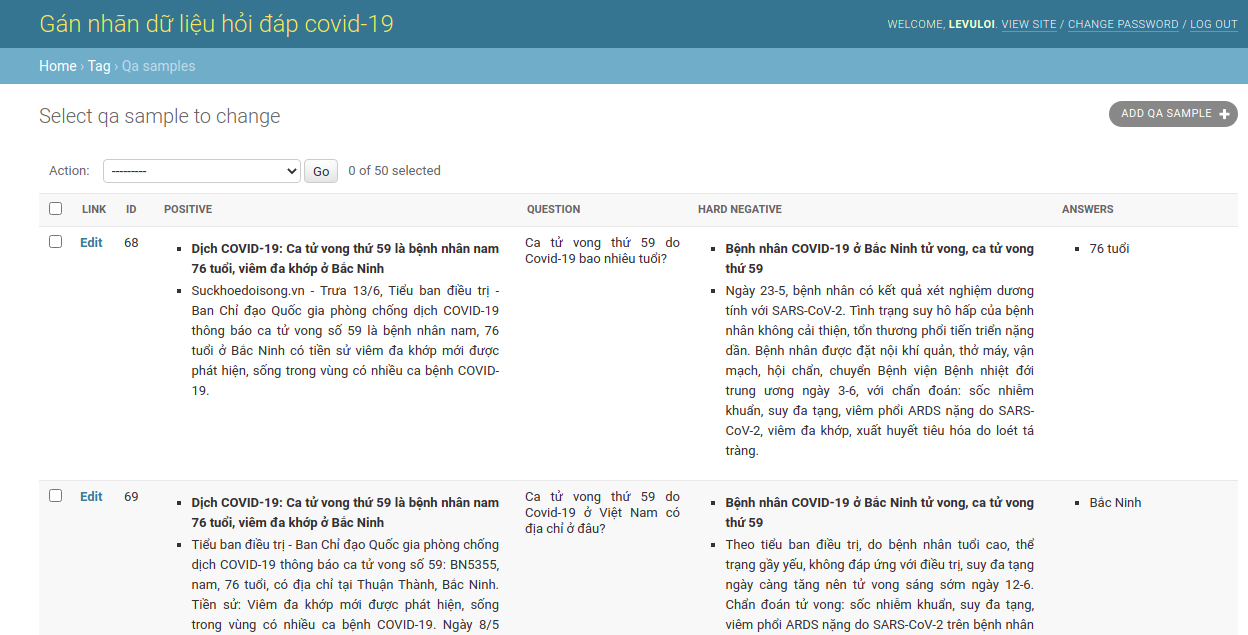
\includegraphics[scale=.25]{images/annotate.png}
\end{frame}
\begin{frame}
\begin{itemize}
	\item Trên hình là một giao diện web em sử dụng để gán nhãn và quản lý dữ liệu được gán nhãn, bao gồm các trường thông tin tương ứng như em đã trình bày trong slide trước.
\end{itemize}
\end{frame}
%====================================
%\subsection{Pretrained model}
%\begin{frame}
%	\frametitle{Pretrained model}
%	\begin{adjustwidth}{0em}{5em}
%	\begin{itemize}
%		\item Vietnamese open-domain question answering for COVID-19 topic was trained from the pretrained language model {\tt NlpHUST/vibert4news-base-cased} pulling from \href{https://huggingface.co/}{\tt huggingface}
%		\item Another well-known pretrained language model for Vietnamese is {\tt PhoBERT} of VinAI, which can also be found on \href{https://huggingface.co/}{\tt huggingface}
%	\end{itemize}
%	\end{adjustwidth}
%\end{frame}
%====================================
\section{Experimental results}
\begin{frame}
	\frametitle{Datasets}
	\begin{itemize}
		\item Google Natural Question: preprocessed data taken from \cite{dpr}
		\begin{itemize}
			\item 58,880 training samples
			\item 8,757 development samples
			\item 3,610 test samples
			\item Context source contains 21,015,324 contexts
			\item To rapidly produce experiments, the context source is reduced to 700,000 contexts and 450 additional contexts are considered to cover all input questions in the test set. 
		\end{itemize}
		\item Vietnamese COVID-19 datatset
		\begin{itemize}
			\item 995 training samples
			\item Context source contains 168,388 contexts
		\end{itemize}
	\end{itemize}
\end{frame}
\begin{frame}
\begin{itemize}
	\item Em xin đi vào phần thứ 5 của bài trình bày đó là phần kết quả thực nghiệm
	\item Bộ dữ liệu mà em sử dụng cho phần thực nghiệm là bộ Google natural question, đã được tiền xử lý, lấy từ nghiên cứu số 2. Tập dữ liệu bao gồm 58880 mẫu dữ liệu huấn luyện, 8757 mẫu dữ liệu development và 3610 mẫu dữ liệu test. Kho văn bản bộ dữ liệu sử dụng bao gồm 21 triệu văn bản khác nhau.
	\item Đây là một kho văn bản có kích thước cực kỳ lớn và để có thể thực nghiệm số lượng lớn thì em đã thu gọn kích thước của kho văn bản xuống  còn 700000, đảm bảo rằng kho văn bản mới luôn chứa văn bản positive cho tất cả các câu hỏi trong tập test. Một phần nhỏ câu hỏi dữ liệu trong tập test (khoảng 450 câu) không có văn bản positive tương ứng trong tập test sẽ được em gán nhãn thủ công và bổ sung.
\end{itemize}
\end{frame}
%=======================================
\begin{frame}
	\frametitle{Metrics}
	\begin{itemize}
		\item Top-$k$ hit scores
		\begin{itemize}
			\item Measure retriever's accuracy
			\item Top-$k$ hit is reached if at least one of $k$ contexts returned by the retriever contains answer(s) for input question. 
		\end{itemize}
		\item Exact match
		\begin{itemize}
			\item Measure reader's accuracy
			\item Measure end-to-end system's accuracy
			\item An exact match hit is reached if answer(s) produced by the open-domain question answering system matches exactly the ground truth answer(s)
		\end{itemize}
	\end{itemize}
\end{frame}
\begin{frame}
\begin{itemize}
	\item Về độ đo sử dụng, em sử 2 độ đo. Độ đo thứ nhất là top-k hit, đo độ chính xác của retriever. retriever sẽ nhận được một điểm top-k hit nếu ít nhất một trong số k văn bản mà nó trả về có chứa câu trả lời cho câu hỏi đầu vào.
	\item Độ đo thứ 2 là exact match, đo độ chính xác của reader cũng độ chính xác của toàn bộ mô hình. Mô hình nhận một điểm exact match nếu câu trả lời nó dự đoán trùng khớp với câu hỏi ground truth.
\end{itemize}
\end{frame}
%=======================================
\begin{frame}
	\frametitle{System settings}
	\begin{adjustwidth}{-2em}{0em}
		\begin{itemize}
			\item Using Google Cloud Platform
			\item Training and inference on Cloud TPUs
			\item Process data on VM Compute Engine
		\end{itemize}
		\vspace{1cm}
		\begin{table}[!htbp]
			\centering
			\caption{Hardware configurations}
			\begin{tabular}{p{.45\linewidth}p{.45\linewidth}}
				\toprule
				Cloud TPUs & VM Compute Engine \\
				\midrule
				\begin{minipage}{6cm}
					TPU v3-8 on-demand:
					\begin{itemize}
						\item TPU version 3
						\item 8 TPU cores
						\item 16GiB memory / TPU core
					\end{itemize}
				\end{minipage} & \begin{minipage}{6cm}
					\begin{itemize}\item OS: Ubuntu 20.04  \item Disk: 30GB \item RAM: 16GB \item nCPUs: 4\end{itemize}
				\end{minipage} \\
				\bottomrule
			\end{tabular}
		\end{table}
	\end{adjustwidth}
\end{frame}
\begin{frame}
\begin{itemize}
	\item Về thiết lập phần cứng, đồ án sử dụng huấn luyện mô hình trên Google Cloud TPU, với đặc điểm là tốc độ huấn luyện nhanh gấp nhiều lần so với khi sử dụng đồng thời nhiều GPU. Việc xử lý dữ liệu cũng được thực hiện trên các máy Compute Engine của Google.
\end{itemize}
\end{frame}
%=======================================
\begin{frame}
	\frametitle{Results on dense retriever}
	\begin{adjustwidth}{-2em}{0em}
		\begin{itemize}
			\item Experimental results on dense retriever are conducted using Google Natural Question dataset.
			\item The proposed method was compared to the baseline in \cite{dpr}
		\end{itemize}
		\begin{figure}
			\begin{minipage}{.45\linewidth}
				%\raggedright
				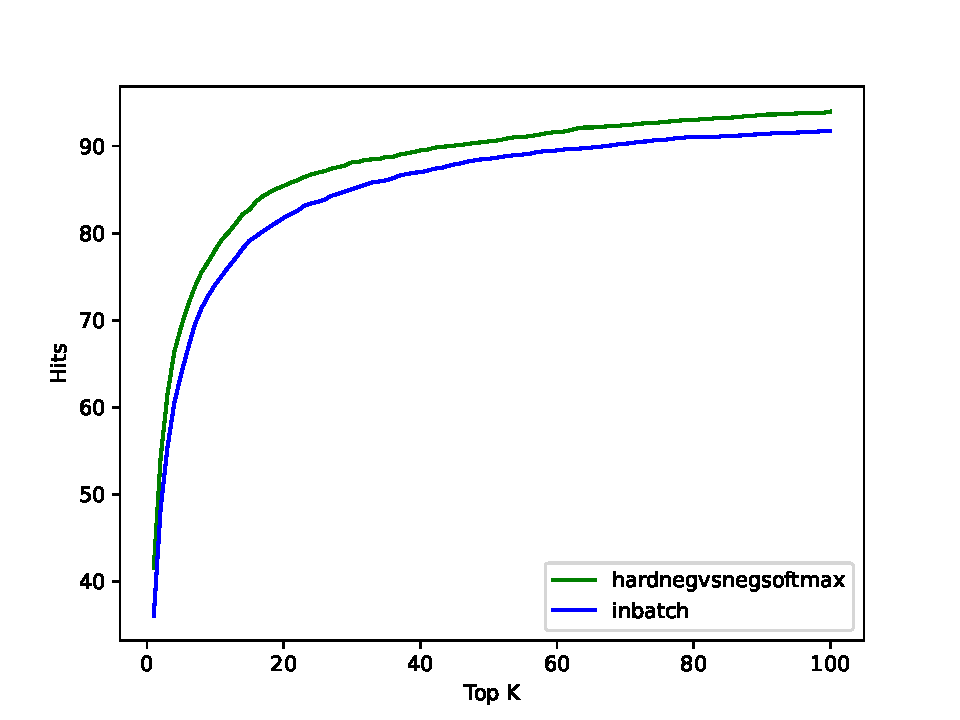
\includegraphics[scale=.32]{images/PDF/experiments/inbatch_hardnegvsnegsoftmax_4-1-5.pdf}
				\caption{\fontsize{8pt}{\baselineskip}\selectfont Comparasion results with baseline model implemented}
			\end{minipage}
			\hfill
			\begin{minipage}{.45\linewidth}
				\raggedleft
				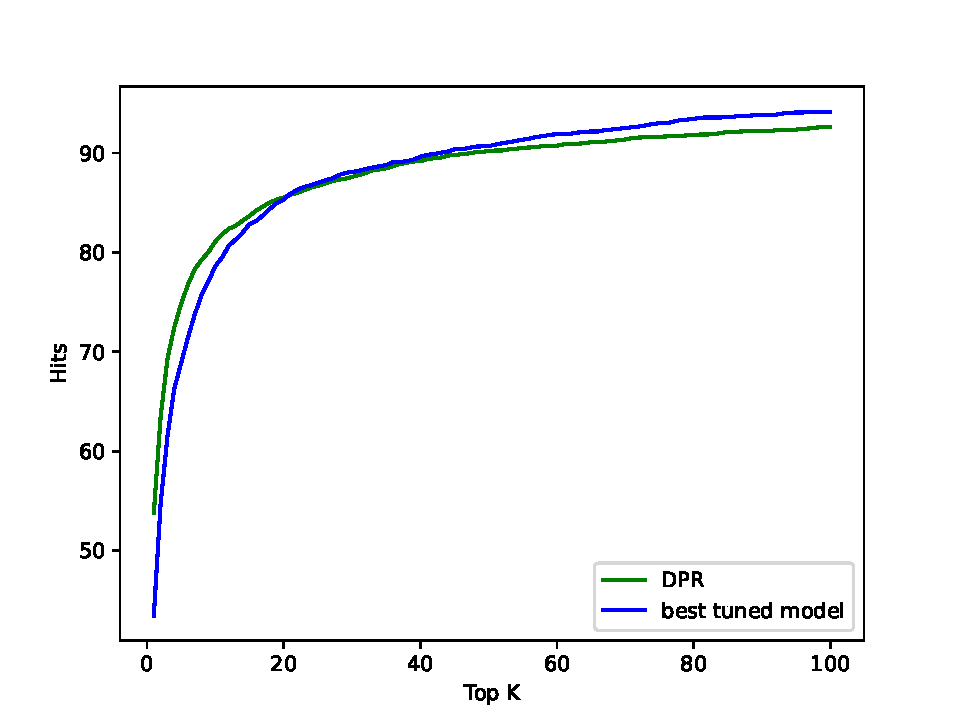
\includegraphics[scale=.32]{images/PDF/experiments/benchmark_compare.pdf}
				\caption{\fontsize{8pt}{\baselineskip}\selectfont Comparasion results with baseline model taken from released checkpoint}	
			\end{minipage}
		\end{figure}
	\end{adjustwidth}
\end{frame}
\begin{frame}
\begin{itemize}
	\item Biểu đồ dưới đây thể hiện kết quả của mô hình mà em đã đề xuất trong phần 3. Hình bên trái là kết quả so sánh giữa mô hình baseline sử dụng trong nghiên cứu số 2 với đề xuất của em khi em tự implement lại mô hình baseline. Như có thể thấy mô hình đề xuất tương ứng với đường màu xanh lá cây có độ chính xác vượt trội hơn hẳn so với mô hình gốc. Ở hình bên phải là kết quả so sánh giữa mô hình đề xuất do em tự code với kết quả chạy khi sử dụng checkpoint mà tác giả bài báo cung cấp. Khi k nhỏ (khoảng nhỏ hơn 20) thì kết quả của checkpoint cao hơn mô hình đề xuất của em, còn với k lớn (lớn hơn 20) thì mô hình đề xuất của em đã dần dẫn tỏ ra tốt hơn. 
\end{itemize}
\end{frame}
%=======================================
%\begin{frame}
%\frametitle{Results on extractive reader}
%\begin{itemize}
%	\item Experimental results on extractive reader are conducted using Google Natural Question.
%	\item Exact match score: 56.6\%
%\end{itemize}
%\end{frame}
%=======================================
%\subsection{Web demo}
%\begin{frame}
%\frametitle{Question Answering about COVID-19}
%\begin{adjustwidth}{-2em}{-2em}
%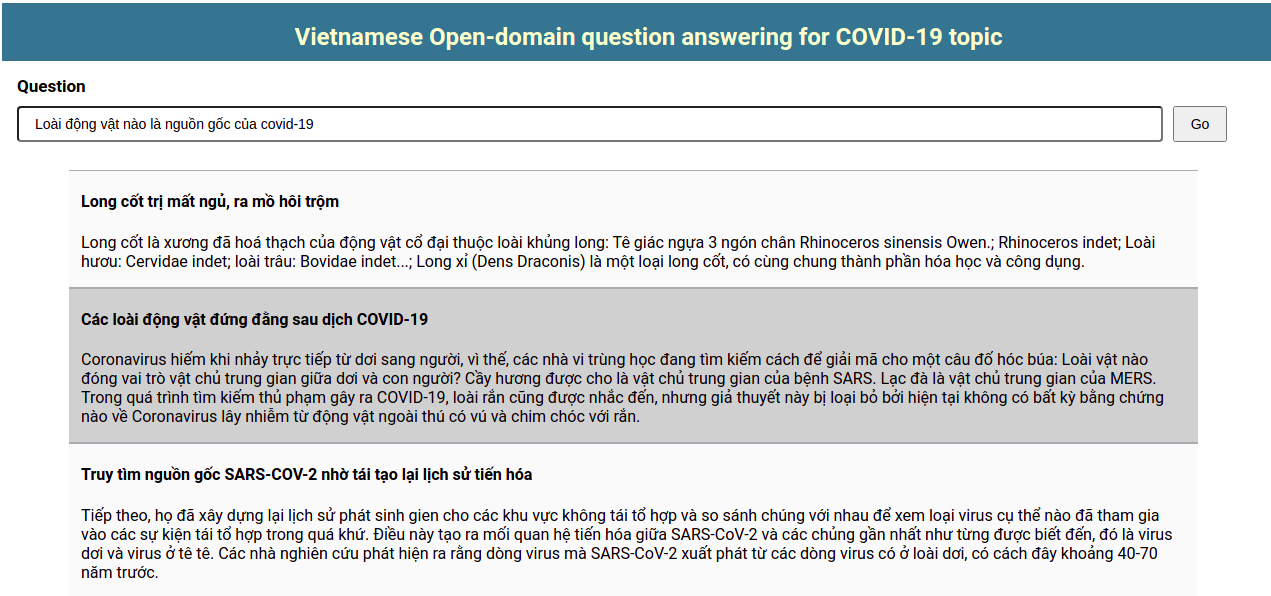
\includegraphics[scale=.27]{images/VNQA.png}
%\end{adjustwidth}
%\end{frame}
%=======================================
\begin{frame}
	\frametitle{Demo: Question Answering about COVID-19}
	\begin{adjustwidth}{-2em}{-2em}
		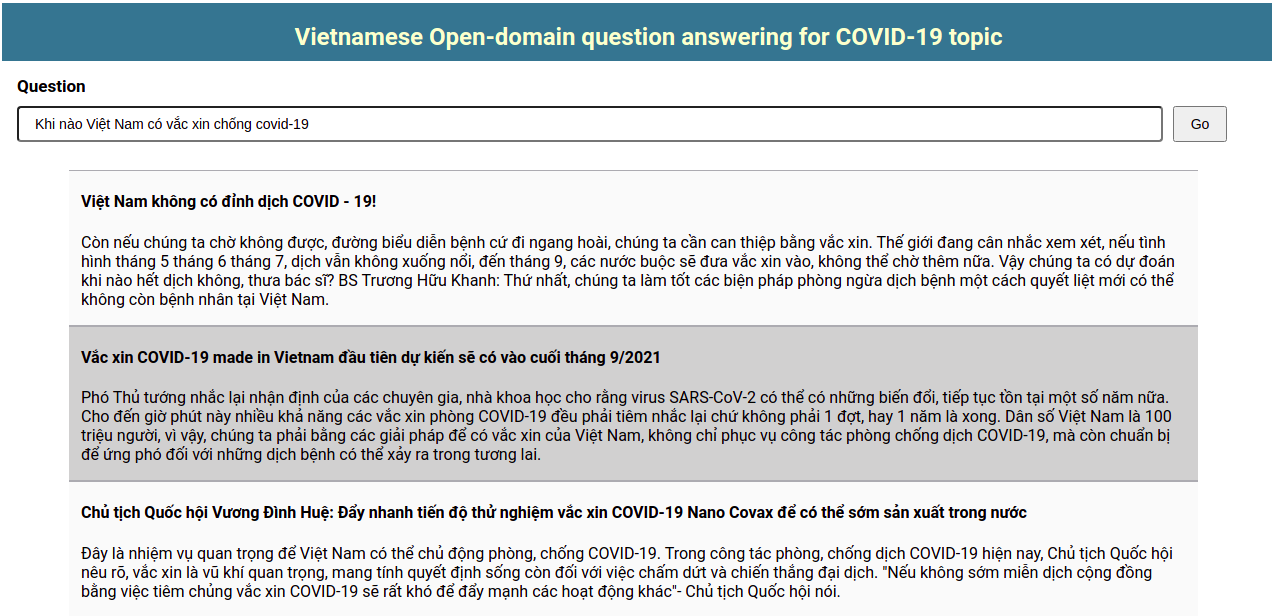
\includegraphics[scale=.27]{images/VNQA_2.png}
	\end{adjustwidth}
\end{frame}
\begin{frame}
\begin{itemize}
	\item Trên đây là hình ảnh demo khi chạy hệ thống cho dữ liệu chủ đề covid-19. Có thể thấy kthi hỏi câu hỏi "Khi nào Việt Nam có vắc xin chống covid-19" thì hệ thống đã trả về các câu hỏi rất có liên quan tới câu hỏi đã cho.
\end{itemize}
\end{frame}
%=======================================
\section{Conclusion and future works}
\begin{frame}
	\frametitle{Conclusion and future works}
	\begin{center}
		\begin{itemize}
			\item Conclusion
			\begin{itemize}
				\item Propose to train retriever model with stratified loss
				\item Conduct a case study for open-domain question answering system in Vietnamese language for COVID-19 topic
				\item Use Cloud TPUs to train large retriever model in short time
			\end{itemize}
			\item Future works
			\begin{itemize}
				\item Study machine reading comprehension problem to improve reader component
				\item Study the relationship between open-domain question answering and automatic knowledge graph construction
			\end{itemize}
		\end{itemize}
	\end{center}
\end{frame}
\begin{frame}
\begin{itemize}
	\item Phần cuối em xin đưa ra kết luận và hướng phát triển.
	\item Tổng kết về các kết quả đã được trong đồ án thì thứ nhất, đồ án đã đề xuất huấn luyện thành phần retriever của hệ thống open-domain question answering với hàm stratified loss, hiệu quả của đề xuất được chứng minh thông qua thực nghiệm.
	\item Thứ hai, đồ án thực hiện một case study của hệ thống open-domain question answering cho dữ liệu tiếng việt với chủ đề về dịch bệnh covid-19.
	\item Thứ 3, trong đồ án em cũng đã tìm hiểu và sử dụng TPU để huấn luyện các mô hình kích thước lớn, giảm thiểu đáng kể tài nguyên tính toán bao gồm CPU cũng như GPU so với nghiên cứu trước đó mà em tìm hiểu.
\end{itemize}
\end{frame}
%=======================================
\begin{frame}[plain]
	%\frametitle{Question Answering about COVID-19}
	\begin{center}
		\textcolor{blue}{\fontsize{20pt}{\baselineskip}\selectfont\bfseries Thank you for your attention}
	\end{center}
\end{frame}
\end{document}